\chapter{Arbejdsmetoder}\label{kapitel_Arbejdsmetoder}
Under projektarbejdet har gruppen benyttet sig af en række arbejdsmetoder til styring og udvikling.
Her beskrives disse metoder samt en opremsning af de udviklingsværktøjer, gruppen har benyttet.

\section{Projektstyring}
Projektets udførsel er inspireret af Scrum.\\
\newline
Alle gruppens medlemmer har i starten af udviklingen underskrevet en samarbejdsaftale (se bilag nr. XX). Denne sikrer enighed omkring udviklingen og definering af kravene. \\
\newline
Der er udviklet en tidsplan til gennemførsel af projektet. Denne er udviklet efter ASE-modellen, men efter en agil tankegang, hvor tidsplanen kan skydes i forhold til, hvilke ændringer og krav der kommer. (???). Tidsplanen bruges til styring af projektet, således at slutproduktet nås i tid til at kunne lave en fuldbyrdig accepttest og for at sikre afleveringsdatoen. 

\begin{figure}[H]
\centering
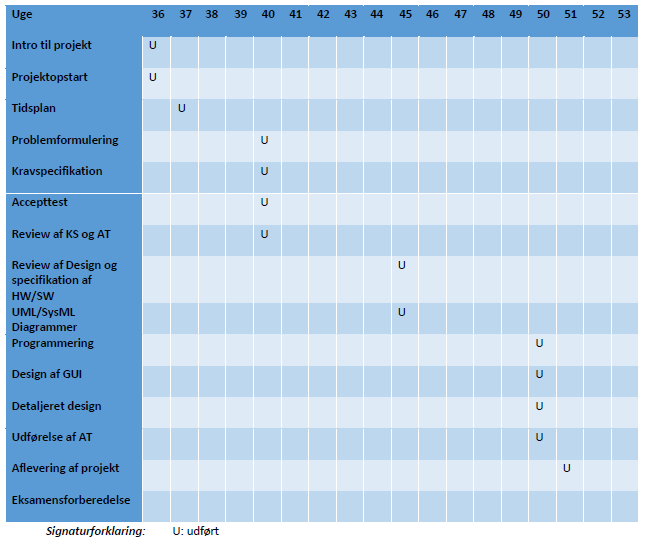
\includegraphics[scale=0.70]{tidsplan.PNG}
\caption{Tidsplan}
\end{figure}

Brugen af Scrum ses i Pivotal Tracker (PT), hvor alle delopgaverne angives som sprints og gruppens medlemmer, enten individuelt eller i mindre enheder, kan "starte" en opgave, og "afslutte" når denne er færdig. Delopgaverne er i hovedtræk angivet med deadlines i tidsplanen, og er i PT prioriteret og markeret med opgavens størrelse fra 1-5. For at kunne følge med i udviklingen og se tilbage på hvilke gruppemedlemmer der udviklede hvilke delopgaver, er der tilføjet en eller flere ansvarlige for delopgaverne. 

\section{Udviklingsproces}
Projektets udviklingsproces er inspireret af agile metoder, som er en fleksibel og tilpasningsdygtig metode. Projektet foretages i små sprints, hvilket kræver meget kommunikation gruppen imellem. Den agile udviklingsproces giver en fleksibilietet i forhold til ændringer der kommer i løbet af gennemførelsen, hvilket har været nødvendigt i projektet, specielt i software-udviklingen.\\
\newline
Mere specifikt er projektet udviklet vha. den agile ASE proces. ASE-modellen er en semi-iterativ udviklingsproces, som drives af UC's, specificeret i kravspecifikationen i startfasen af projektet. ASE-modellen er inspireret af vandfaldsmodellen, hvor projektet ligeledes inddeles i faser, udvikles step for step og testes, og V-modellen, hvor der testes efter hver fase, og det derfor er nemmere at finde eventuelle fejl i løbet af udviklingen.\\
\newline
Vandfaldsmodellen er specifikt brugt i starten af projektets udvikling, hvor denne inddeles i steps. Disse steps blev udviklets af gruppen som samlet enhed, og indebærer bl.a. problemformulering, UC's, krav, accepttest og tidsplan. Efter denne specifikation af projektet, er gruppen delt op i to, en hardware- og en softwaregruppe.

\begin{figure}[H]
\centering
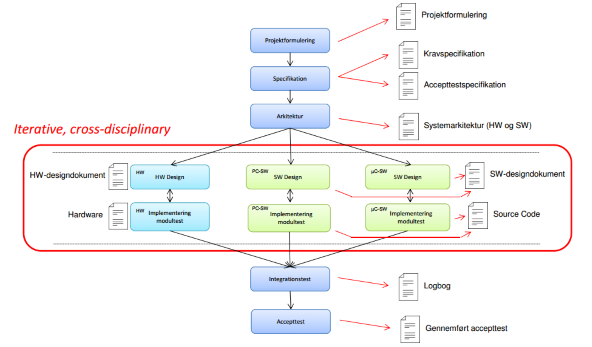
\includegraphics[scale=0.80]{ase.PNG}
\caption{ASE-modellen}
\end{figure}

V-modellen er brugt i test af software, i hht. integrationstest og modultests og en accepttest for kunden (gruppens vejleder) af hele systemet. \\
\newline
For at sikre at ingen af projektets dokumenter mistes, er der brugt delingsværktøjet Github. Her gennem dokumenterne i en individuel mappe på hver af gruppemedlemmernes computere og i "skyen". Github gemmer en versionshistorik af ændringer i dokumenterne, som angives heri.  

\section{Udviklingsværktøjer} %*Hed før redskaber
I udviklingen og implementeringen af projektet, er følgende udviklingsværktøjer anvendt:
\subsubsection{DAQ:}
USB-device fra National Instrument. Bruges til at opsamle data som vha. konvertering danner et digitalt signal.
\subsubsection{Analog Discovery:}
Generer et analogt signal ud fra blodtryksdata. Dette analoge signal konverteres, vha. DAQ'en, til et digitalt signal.
\subsubsection{WaveForms:}
Bruges sammen med Analog Discovery og DAQ'en til at indsende data til programmet (???)
\subsubsection{Visual Studio:}
Visual studio er et udviklingsværktøj til software. Dette program er anvendt til at designe software-delen. Programmeringssproget, der er anvendt her, er C$\#$. 
\subsubsection{Microsoft Visio:}
Microsoftprogram til udvikling af hardware-/software diagrammer. Anvendes til at forenkle komplekse oplysninger via enkle, letforståelige diagrammer.
\subsubsection{Multisim:}
Til design af hardware komponeneter til forstærkeren er simuleringsværktøjet Multisim anvendt. 
\subsubsection{Ultiboard:}
Til udlægning af print er programmet Ultiboard benyttet. Det er godt integreret med Multisim, og var derfor det oplagte valg.
\subsubsection{Github:}
Github er et delingsværktøj, som automatisk opretter et versionshistorik. Denne er derfor anvendt til dokumentdeling igennem projektet. 
\subsubsection{Pivotal Tracker:}
Pivotal tracker er anvendt som scrumboard til at styre projektets løbende arbejdsopgaver. 
\subsubsection{Mathad:}
Matchad er et regneværktøj, som er anvendt til at udføre beregner i Hardware-delen. 
\subsubsection{Latex:}
Latex er et såkaldt opmærkningssprog, som er velegnet til rapportskrivning, derfor er dette valgt til projektrapporten. 

\section{Rollefordeling}
\subsubsection{Mødestruktur}
Gruppen har ved projektetsstart, i samarbejde med vejlederen, fastlagt den overordnede mødestruktur. Projektgruppen er i udviklingen af hardware og software inddelt i to undergrupper - en hardwaregruppe og en softwaregruppe. Der er fastlagt et ugentligt møde med vejleder, planlagt efter hvordan ugen forløber, og mindst et ugentligt møde HW- og SW grupperne imellem. Møder  undergrupperne imellem, er fastlagt efter behov, men også mindst én gang ugentligt. I perioder har dette været et møde i ugen, andre 4-5 møder i ugen. Kravene til møderne er defineret i samarbejdskontrakten (bilag XX). \\
\newline
Møder med vejleder er aftalt over mail fra gang til gang, hvor også en dagsorden er sendt med. Denne danner grundlag om mødet og sikrer, at alle punkter gennemgåes. Møder gruppen imellem aftales efter hvert enkelt møde, hvor der også her har været udviklet en dagsorden - dog kun til de møder, hvor denne har givet mening.\\
\newline
Der er lavet mødereferater for samtlige møder med vejleder og for reviews med andre projektgrupper. Derudover er der lavet logbøger ved samtlige møder gruppemedlemmerne imellem, både samlet og i undergrupperne. Mødereferaterne og logbøgerne sikrer at beslutningerne, taget ved de forskellige møder, altid kan refereres tilbage, hvorfor der ikke opstår tvivl om hvorvidt beslutningen blev taget, af hvem og hvad der overordnet blev argumenteret for.\\
Mødereferater og logbøger er skrevet i hvert sit dokument i Latex (bilag XX), hvor de hver især er angivet med mødenummer, dato, referent og tilstedeværende gruppemedlemmer.  

\subsubsection{Deadlines}
Der har fra projektets start været deadlines til dele af projektet. Disse har af overordnet karakter været angivet fra IHA's side, hvor gruppen, ud fra tidsplanen, har angivet flere og mere detaljerede deadlines for at sikre stabil fremgang i projektets gennemførsel. \\
Den første, og yderst væsentlige, deadline bestod af kravpecifikation og accepttest, som det også ses i tidsplanen (bilag X). Disse dokumenter udvikledes af projektgruppen som samlet enhed, hvor gruppen arbejde i fællesskab om at definere projektets krav i hht. løsningen af problemet. Kravspecifikation og accepttest udviklet parallelt, i og med at disse skal stemme fuldstændig overens. \\
\newline
Ligeledes har der været deadlines i forhold til design og implementering, som bruges til design og beskrivelse af projektet.\\
\newline
Den sidste overordnede deadline består af accepttest, hvor hele systemet testes i hht. projektets definerede krav. Dette gøres sammen med kunden, som i dette tilfælde er vejlederen. 

%SKAL DER FLERE DEADLINES IND? 

\subsubsection{Review}

